\documentclass[11pt]{article}
\usepackage{latexsym}
\usepackage{amsmath}
\usepackage{amssymb}
\usepackage{amsthm}
\usepackage{epsfig}
\usepackage[tight]{subfigure}
\usepackage{hyperref}

\usepackage{amsmath}

\usepackage{helvet}   %Required
\usepackage{courier}  %Required
\usepackage{url}      %Required
\usepackage{xcolor}
\usepackage{pifont}% http://ctan.org/pkg/pifont
\usepackage{booktabs}
\usepackage{multirow}
% \usepackage{subcaption}

\DeclareMathOperator*{\minimize}{min}
\DeclareMathOperator*{\maximize}{max}

\DeclareMathOperator*{\argmax}{argmax} % thin space, limits underneath in displays
\DeclareMathOperator*{\argmin}{argmin}

\usepackage{algorithm}
 %on linux you may need to run sudo apt-get install texlive-full to install algorithm.sys
\usepackage{algorithmic}

\usepackage{verbatim}

\newcommand{\handout}[5]{
  \noindent
  \begin{center}
  \framebox{
    \vbox{
      \hbox to 5.78in { {#1} \hfill #2 }
      \vspace{4mm}
      \hbox to 5.78in { {\Large \hfill #5  \hfill} }
      \vspace{2mm}
      \hbox to 5.78in { {\em #3 \hfill #4} }
    }
  }
  \end{center}
  \vspace*{4mm}
}

\newcommand{\lecture}[5]{\handout{#1}{#2}{#3}{#4}{#5}}
\newcommand{\collision}[0]{\mathrm{collision}}
\newcommand{\nocollision}[0]{\overline{\collision}}

\newcommand*{\QED}{\hfill\ensuremath{\square}}

\newtheorem{theorem}{Theorem}
\newtheorem{corollary}[theorem]{Corollary}
\newtheorem{lemma}[theorem]{Lemma}
\newtheorem{observation}[theorem]{Observation}
\newtheorem{proposition}[theorem]{Proposition}
\newtheorem{definition}[theorem]{Definition}
\newtheorem{claim}[theorem]{Claim}
\newtheorem{fact}[theorem]{Fact}
\newtheorem{assumption}[theorem]{Assumption}
\newtheorem{note}[theorem]{Note}

% 1-inch margins, from fullpage.sty by H.Partl, Version 2, Dec. 15, 1988.
\topmargin 0pt
\advance \topmargin by -\headheight
\advance \topmargin by -\headsep
\textheight 8.9in
\oddsidemargin 0pt
\evensidemargin \oddsidemargin
\marginparwidth 0.5in
\textwidth 6.5in

\parindent 0in
\parskip 1.5ex
%\renewcommand{\baselinestretch}{1.25}


%%%%% Customize command %%%%%
\newcommand{\btheta}{\boldsymbol{\theta}}
\newcommand{\bz}{\boldsymbol{z}}
\newcommand{\bw}{\boldsymbol{w}}
\newcommand{\bu}{\boldsymbol{u}}
\newcommand{\bv}{\boldsymbol{v}}
\newcommand{\xmark}{\ding{55}}

\begin{document}

\lecture{Statistical Techniques in Robotics (16-831, S21)}{Lecture \#16
  (Wednesday, March 31)}{Lecturer: Kris Kitani}{Scribes: Chih-Wei Wu, Yu-Jhe Li}{Model-based Value-based RL}

\section{Review}

In the previous course, we have introduced the general sequence feedback learning problem and we will review these concepts in this section. Generally, most of the contents in this document are from course materials~\cite{16831lecture16}.

\subsection{Sequence Feedback Learning Problem}
Before we move into the RL problems that are
sequential, evaluative, and sampled, we first review some of the learning problem we learned in the Table~\ref{table:decision}. Difference of these problems are summarized as follows:
\vspace{-3mm}
\begin{itemize}\itemsep -2pt
    \item \textbf{Instructive} problems (PWMA,OLC): Observe the fully observable loss, update all your predictor parameters.
    
    \item \textbf{Sampled-evaluative} problems (MAB, C-MAB): observe the partially observable loss, update one (arm) predictor parameter at a time.
    
    \item \textbf{Sequential} problems (RL): Obtain a sequence of rewards, update your future predictor (value function), then update action predictor (policy).
\end{itemize}

\begin{table}[H]
\begin{center}
  \caption{Decision-making problems covered so far}
  \label{table:decision}
  \begin{tabular}{c|ccc}
  \toprule
  Problem & Sampled & Evaluative & Sequential\\
  \midrule
  PWMA & \xmark & \xmark & \xmark\\
  OLC & \checkmark & \xmark & \xmark\\
  MAB & \xmark & \checkmark & \xmark\\
  C-MAB & \checkmark & \checkmark & \xmark\\
  \midrule
  RL & \checkmark & \checkmark & \checkmark\\
  \bottomrule
  \end{tabular}
 \end{center}
 \vspace{-5mm}
\end{table}


\subsection{Sequential Decision Making and Markov Decision Process}
We have different ways to decompose a temporal sequence of variables such as:
\vspace{-5mm}
\begin{itemize}\itemsep -2pt
    \item Bayesian Bandit:
    $p(r_0,...,r_T|a_0,...,a_T,\theta) = \prod_{t=0}^{T} p(r_t|a_t,\theta)$
    \item Dynamic Bayesian Network:
    $p(x_0,...,x_T,e_1,...,e_T) = p(x_0)\prod_{t=0}^{T} p(x_{t+1}|x_t)p(e_t|x_t)$
\end{itemize}
Today, we introduce the \textbf{Markov Decision Process}:
$$p(s_0,...,s_T,a_0,...,a_T) = p_0(s_0) \prod_{t=0}^{T-1} p(s_{t+1}|s_t,a_t)p(a_t|s_t)$$

A Markov Decision Process (MDP) can be used as a framework to formulate and solve reinforcement learning problems. In MDP, we define some of the important notations as: state $s\in S$, action $a \in A$, state transition dynamics $p(s'|s,a)$, reward function $r(s',s,a)$, state prior $p_0(s)$, policy $\pi(a|x)$, and discount factor $\gamma$. Policy describes which action to take in a given state. State transition dynamic describes the probability of transition to another state. Reward function maps a state to a real value. The graphical model is presented in the Figure~\ref{fig:MDPgraph}.

\begin{figure}[H]
    \centering
    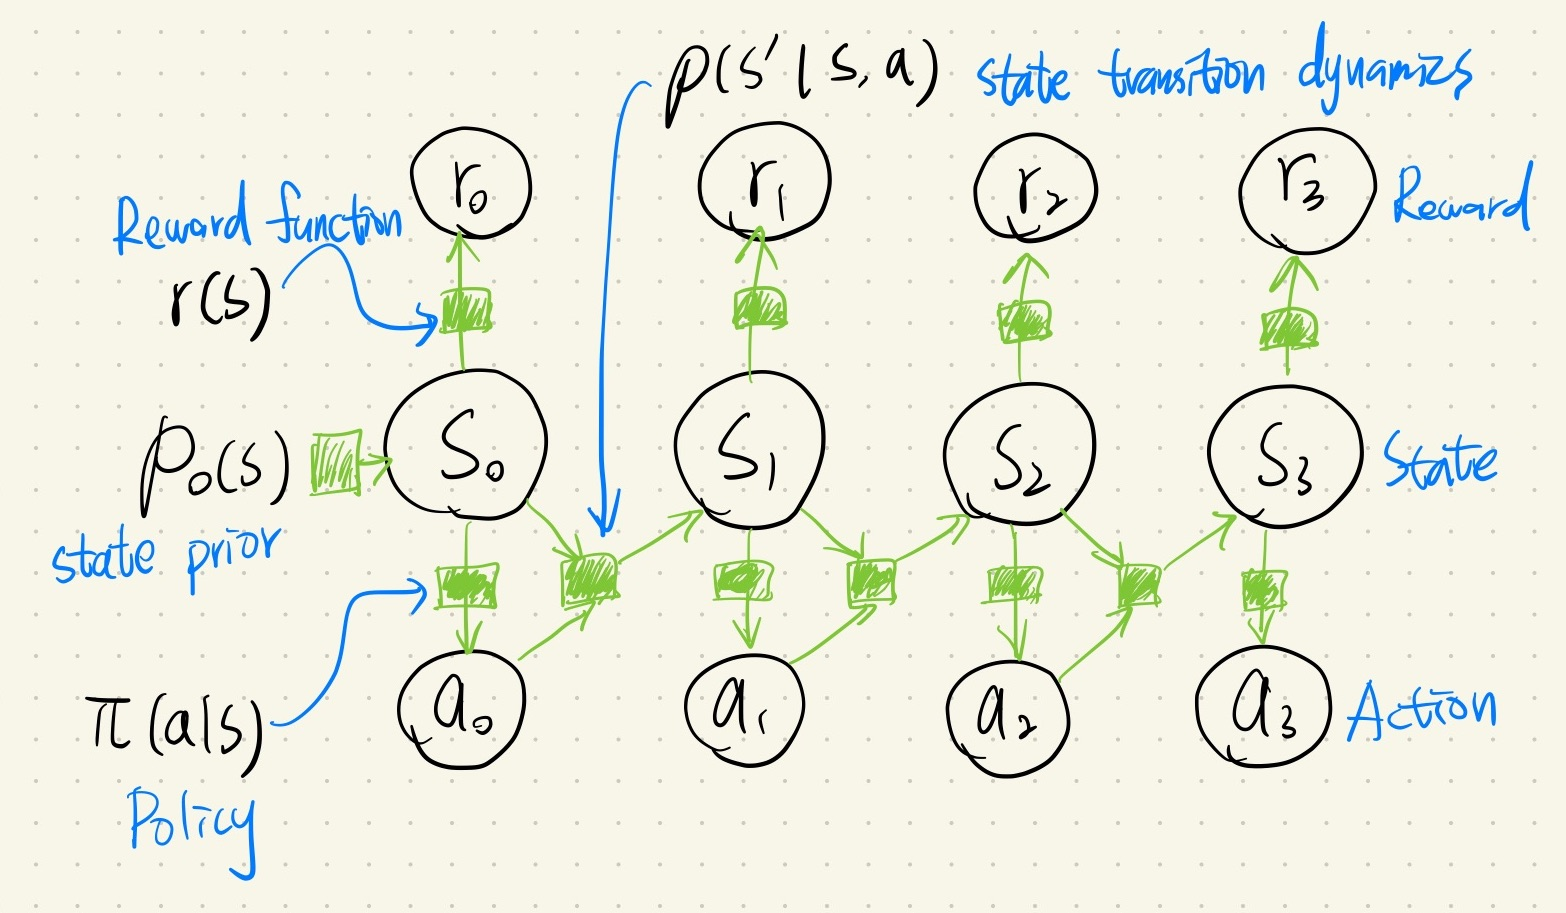
\includegraphics[width=0.8\textwidth]{Img/MDP_graph.jpg}
    \caption{Graphical model of MDP.}
    \label{fig:MDPgraph}
\end{figure}

\subsection{Value function in MDP}\label{sec:mdp_value}
We define the total expected return of a trajectory starting in state $s$ as \textbf{state value function}:
$$V^{\pi}(s) = \mathbb{E}_p [r_0+r_1+r_2+...|s_0=s],$$
where the reward is defined as:
$$r_t \triangleq r(s_{t+1}=s',a_t=a,s_t=s).$$
By a discount factor $\gamma = [0,1]$, we can also define the infinite horizon discounted return as:
$$V^{\pi}(s) = \mathbb{E}_p [\gamma^0 r_0 + \gamma^1 r^1+\gamma^2 r^2+...|s_0=s].$$

The total expected return of a trajectory starting in state $s$ and taking action $a$ is defined as \textbf{state-action value function}:
$$Q^{\pi}(s,a) = \mathbb{E}_p [\gamma^0 r(s_0) + \gamma^1 r(s_1)+\gamma^2 r(s_2)+...|s_0=s,a_0=a].$$
% \subsection{Value function}
The relationship between state value function ($V$) and state-action value function ($Q$) is:
$$V^{\pi}(s) = \sum_a \pi (a|s) Q^{\pi} (s,a)$$

\section{Summary}
\subsection{MDP Concepts}
We have reviewed the value functions in the section~\ref{sec:mdp_value}. Now we are going to introduce more concepts in the MDP which include the Bellman equation and the Bellman Optimality Equations.
 

\subsubsection{The Bellman equation}
Now we would like to make the value function to be recurrent. That is, the recursive relationship between state value functions under a given policy is defined as Bellman equation:
%
$$V^{\pi}(s) = \sum_a \pi(a|s)\sum_{s'} p(s'|s,a) [r(s', a, s) + \gamma V^{\pi}(s')]$$
%
This can be interpreted as taking one step, receiving a reward and see the value of the state where you transition to. The current state value will consider all the possible transitions to neighboring state.
\noindent\textit{Proof:}
\begin{equation}
\begin{split}
V^{\pi}(s_0) = & \mathbb{E} \left[\gamma^0 r_0 + \gamma^1 r_1+\gamma^2 r_2+...\bigg|s_0\right]\nonumber\\    
= & \mathbb{E}\left[\sum_{t=0}^{\infty} \gamma^t r_t\bigg|s_0\right]\\
= & \mathbb{E}\left[r_0+\sum_{t=0}^{\infty} \gamma^t r_t\bigg|s_0\right]\\
= & \sum_{a_0:\infty} \sum_{s_1:\infty} p(s_{1:\infty},a_{0:\infty}) \left[r_0+\sum_{t=0}^{\infty} \gamma^t r_t\bigg|s_0\right]\\
= & \sum_{a_0} \sum_{s_1} p(s_1|s_{0},a_{0})\pi(a_0|s_0) \left\{r_0+ \sum_{a_1:\infty} \sum_{s_2:\infty} p(s_{2:\infty,a_{1:\infty}}) \left[\sum_{t=1}^{\infty} \gamma^t r_t\bigg|s_1\right]\right\}\\
= & \sum_{a_0} \sum_{s_1}p(s_1|s_{0},a_{0})\pi(a_0|s_0) \left\{r_0+ \mathbb{E} \left[\sum_{t=1}^{\infty} \gamma^t r_t\bigg|s_1\right]\right\}\\
= & \sum_{a_0} \pi(a_0|s_0) \sum_{s_1} p(s_1|s_{0},a_{0}) \left\{r_0+ \gamma V^{\pi} (s_1)\right\}\\
\end{split}
\end{equation}
%
The Bellman Equation for state-action value function can also be defined as:
$$Q^{\pi}(s,a) = \sum_{s'} p(s'|s,a) \left\{r(s',a,s) + \sum_{a'} \pi(a'|s') Q^{\pi}(s',a')\right\}$$
\noindent\textit{Proof:}
\begin{equation}
\begin{split}
Q^{\pi}(s_0,a_0) = & \mathbb{E} \left[\gamma^0 r_0 + \gamma^1 r_1+\gamma^2 r_2+...\bigg|s_0,a_0\right]\nonumber\\    
= & \mathbb{E}\left[\sum_{t=0}^{\infty} \gamma^t r_t\bigg|s_0,a_0\right]\\
= & \mathbb{E}\left[r_0+\sum_{t=0}^{\infty} \gamma^t r_t\bigg|s_0,a_0\right]\\
= & \sum_{s_1:\infty} p(s_{1:\infty},a_{0:\infty}) \left[r_0+\sum_{t=0}^{\infty} \gamma^t r_t\bigg|s_0,a_0\right]\\
% = & \sum_{s_1} p(s_1|s_{0},a_{0}) \left\{r_0+ \sum_{a_1:\infty} \sum_{s_2:\infty} p(s_{2:\infty,a_{1:\infty}}) \left[\sum_{t=1}^{\infty} \gamma^t r_t\bigg|s_1\right]\right\}\\
= &  \sum_{s_1}p(s_1|s_{0},a_{0}) \left\{r_0+ \mathbb{E} \left[\sum_{t=1}^{\infty} \gamma^t r_t\bigg|s_1\right]\right\}\\
= &  \sum_{s_1}p(s_1|s_{0},a_{0}) \left\{r_0+ \sum_{a_1} \pi(a_1|s_1)\mathbb{E} \left[\sum_{t=1}^{\infty} \gamma^t r_t\bigg|s_1,a_1\right]\right\}\\
= &  \sum_{s_1} p(s_1|s_{0},a_{0}) \left\{r_0+ \sum_{a_1} \pi(a_1|s_1) Q^{\pi} (s_1,a_1)\right\}\\
\end{split}
\end{equation}
The importance of Bellman equation:
\vspace{-5mm}
\begin{itemize}\itemsep -2pt
\item It defines a (recursive) relationship between value functions
\item It is used to derive the Bellman optimality equation
\item It gives us a useful constraint for optimization
\item It provides the basis for many algorithms to solve for the optimal value function and optimal policy.
\end{itemize}

\subsubsection{The Bellman Optimality Equations}
We can now use these equations to derive the Bellman optimality equations. This gives us a method of comparing policies and can be used to find the best policy. In this case, the policy that results in the agent collecting the maximum reward is regarded as the best policy and it should obtain the greatest expected return.
$$V^{\pi^*}(s) = \max_{\pi} V^{\pi^*}(s)$$
$$Q^{\pi^*}(s,a) = \max_{\pi} Q^{\pi^*}(s,a)$$
Expanding the equations we can get:
$$V^{\pi^*}(s) = \max_{a} \sum_{s'} p(s'|s,a) [r_t + \gamma V^{\pi^*}(s')]$$
$$Q^{\pi^*}(s,a) = \sum_{s'} p(s'|s,a) [r(s)+\gamma \max_{a'} Q^{\pi^*}(s',a')]$$

We can further derive the relationship between $Q$ and $V$ as:
\begin{itemize}
    \item From $Q$ to $V$:
    $$V^{\pi^*}(s) = \max_{a} Q^{\pi^*}(s,a)$$
    \item From $V$ to $Q$:
    $$Q^{\pi^*}(s,a) = \sum_{s'} p(s'|s,a) [r(s)+\gamma V^{\pi^*}(s')]$$
\end{itemize}
\noindent\textit{Proof:}
\begin{equation}
\begin{split}
V^{\pi^*}(s) = & \sum_a \pi (a|s) Q^{\pi^*}(s,a) \nonumber\\  
= & \max_{a} Q^{\pi^*}(s,a)\\
= & \max_{a} \mathbb{E}\left[\sum_{t=0}^{\infty} \gamma^t r_t\bigg|s_0=s,a_0=a\right]\\
= & \max_{a} \mathbb{E}\left[r_0+\sum_{t=0}^{\infty} \gamma^t r_t\bigg|s_0=s, a_0 =a\right]\\
= & \max_{a} \sum_{s'} p(s_1=s'|s,a) \left[r_0+ \mathbb{E} \left\{\sum_{t=0}^{\infty} \gamma^t r_t\bigg|s_1=s' \right\}\right]\\
= & \max_{a} \sum_{s'} p(s'|s,a) [r_t + \gamma V^{\pi^*}(s')]\\
\end{split}
\end{equation}



\subsection{Model-based Prediction and Control}

Recall in Reinforcement Learning, our learning goal is to \textbf{obtain the optimal policy} $\hat{\pi}$ from a data distribution $D(\zeta, R)$. The optimal policy $\hat{\pi}: s \rightarrow a$ is a function that maps a state (or observation $x$) to an action. The data distribution could be sampled to generate a data sample consisting a sequence of observation and actions $\zeta = \{(s_1, a_1), (s_2, a_2), \dots, (s_T, a_T)\}$, and a return value $R_i \in \mathbb{R}$ that tells you how good/bad the entire sequence is. The optimal policy is obtained \textbf{by optimizing for the maximum expected reward}:
%
\begin{align}
\hat{\pi} = \argmax_\pi \mathbb{E}_{p_\pi(\zeta)}\Big[\sum^T_{t=0} r^t \Big].
\end{align}
%
Here, $r^t \triangleq r(s^{t+1}, a^t, s^t)$ is the reward of iteration $t$, consisting the current state $s^t$, the current action $a^t$ and the next state $s^{t+1}$. $\zeta = \{s^{(0)},a^{(0)},s^{(1)},a^{(1)},...,s^{(T)},a^{(T)}\}$ is the state-action sequence. $p_\pi(\zeta) = p(s^0)\prod_{t=0}^T \pi(a^t|s^t)p(s^{t+1}|s^t, a^t)$ is the probability of the entire sequence. 

In previous lecture, we quantify the expected total return of a trajectory starting in state $s$ and taking action $a$ as a \textbf{state-action value function}:
%
\begin{align}
Q^\pi(s, a) = \mathbb{E}_p[\gamma^0 r(s_0) + \gamma^1 r(s_1)+ \dots | s_0 = s, a_0 = a].
\end{align}
%
So the optimization goal could be rewrite as:
%
\begin{align}
\pi(s) = \argmax_a Q(s, a)
\end{align}
%
If we could solve for the value function $Q$, then it is easy to derive the policy. This kind of RL approach is called the \textbf{Value-based RL}. See Figure~\ref{fig:valueRL} for more context. For a value-based RL problem, we are given the following as input:
%
\begin{itemize}
    \item Finite state space $s \in \mathcal{S}$
    \item Finite action space $a \in \mathcal{A}$
    \item Dynamic model $p(s'|s, a)$
    \item Reward function $r(s', s, a)$
\end{itemize}
%
and begin asked to predict the optimal policy. But is it all? Recall the state-action value function is actually characterized by a policy $\pi(a|s)$. However the policy is what we want to solve in the first place. So this could be though as an chicken-and-egg problem. 


\begin{figure}[h]
    \centering
    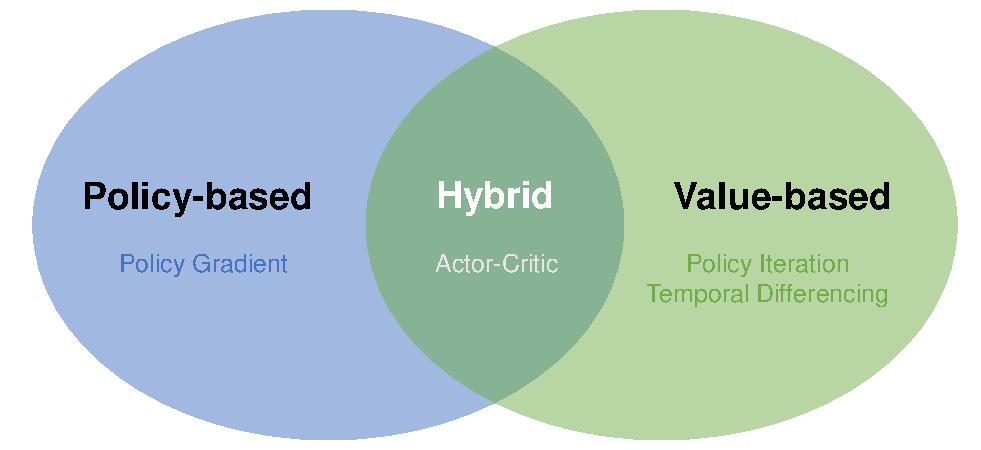
\includegraphics[width=0.6\textwidth]{Img/value-based-RL.pdf}
    \caption{Value-based Reinforcement Learning.}
    \label{fig:valueRL}
\end{figure}


To solve this problem, we typically fix the policy calculated from the last iteration, and solve for the value function. We call this step \textbf{Policy Evaluation}. We then retrieve the policy that maximizes the value function, and use this policy for the next iteration. We term this step as \textbf{Policy Improvement}. We alternate these two steps throughout the algorithm. An illustration of the process is presented in Figure~\ref{fig:value-control}.


\begin{figure}[h]
    \centering
    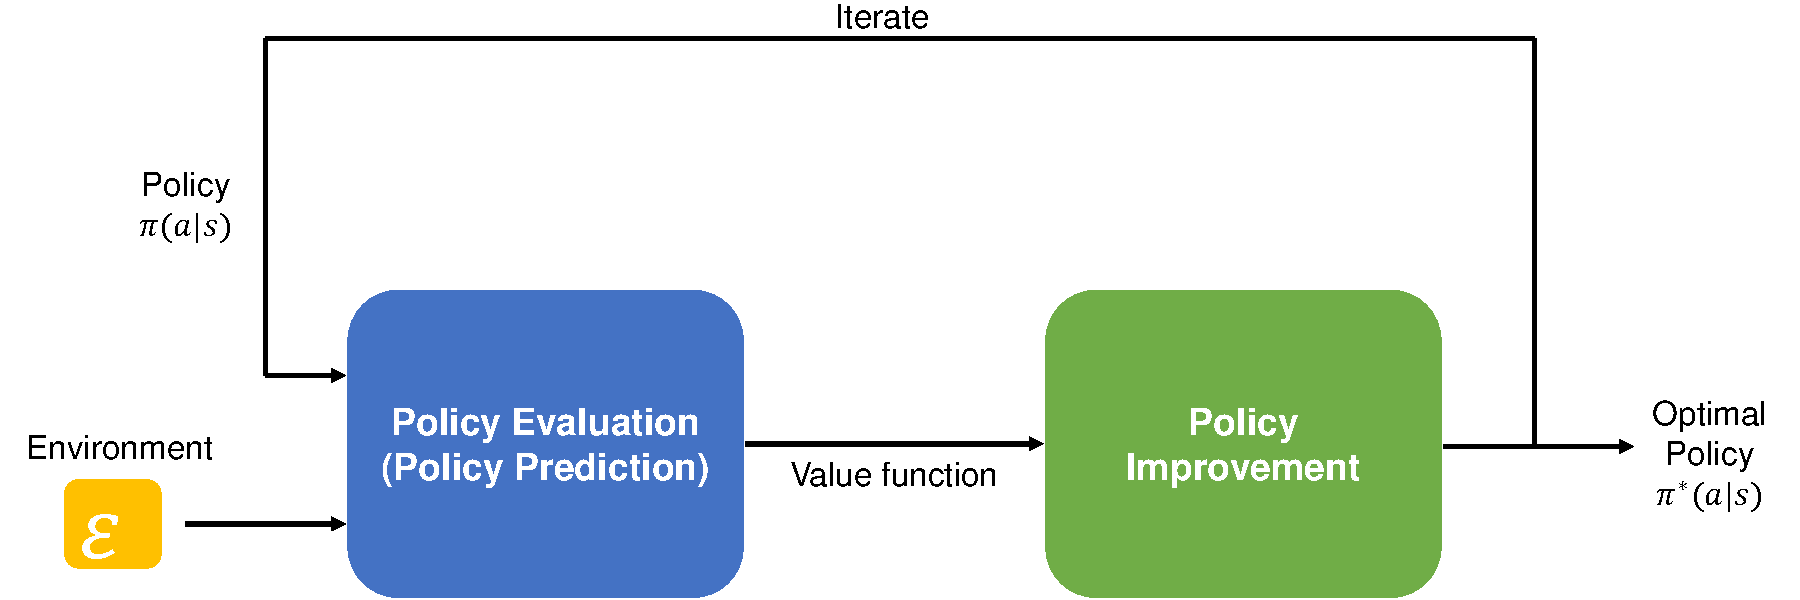
\includegraphics[width=0.8\textwidth]{Img/policy-iteration.pdf}
    \caption{Solving Value-based RL.}
    \label{fig:value-control}
\end{figure}

Depending on the type of environment given to Policy Evaluation step, we can categorize value-based RL into 2 classes:
\begin{enumerate} \itemsep -2pt
    \item The \textbf{model-based} method assumes the state transition dynamics and reward function are known.
    \item The \textbf{model-free} method assumes we do not know anything about the environment, giving the algorithm only sampled feedback. 
\end{enumerate}
 In this section, we will focus on value-based model-based method (a.k.a Policy Iteration).


\subsection{Policy Evaluation}

First, we focus on the Policy Evaluation step for solving value-based model-based RL, as indicated in Figure~\ref{fig:value-control}. For this step, we take policy $\pi(s|a)$, transition dynamics $p(s'|s, a)$ and $r(s', s, a)$ as input, and aims to predict the value function characterized by the Bellman Equation:
%
\begin{align}
V^\pi(s) &= \sum_a \pi(a|s) \sum_{s'} p(s'|s, a)[r(s', a, s) + \gamma V^\pi(s')] \\
&= \sum_a \pi(a|s) Q^\pi (s, a) \label{eq:value_function}
\end{align}
%
We could develop an algorithm for prediction based on this objective:
%
\begin{algorithm}[H]
\caption{Policy Evaluation ($\pi, r(s), p(s'|s, a), \gamma$)}
\label{algo:policy_evaluation}
\begin{algorithmic}[1]
\STATE $V \leftarrow \text{rand}(\mathbb{R})$
\STATE $V' \leftarrow \text{rand}(\mathbb{R})$
\WHILE{$\max_s |V(s)-V'(s)| \geq \epsilon$}
\STATE $V' \leftarrow V$
\FOR{$s \in \mathcal{S}$}
\STATE $Q(s, a) = r(s) + \gamma \sum_{s'} p(s'|s, a) V'(s') \quad \forall a$ \hfill $\triangleright$ This step interact with the environment
\STATE $V(s) = \sum_a \pi(s|a)Q(s, a)$
\ENDFOR
\ENDWHILE
\RETURN Q
\end{algorithmic}
\end{algorithm}


\subsection{Policy Improvement}

For the Policy Improvement step, we take the value function $Q(s, a)$ given by the Policy Evaluation step, and estimate the optimal policy $\pi(a|s)$ for next iteration. Recall that when the policy is optimal, Equation~\ref{eq:value_function} could be rewrite as:
%
\begin{align*}
V^{\pi^*}(s) = \max_a Q^{\pi^*}(s, a),
\end{align*}
%
assuming that the transition of state is deterministic to the action. Then, we write the algorithm for Policy Improvement as follows.
%
\begin{algorithm}[H]
\caption{Policy Improvement ($Q$)}
\label{algo:policy_improvement}
\begin{algorithmic}[1]
\FOR{$s \in \mathcal{S}$}
\STATE $\pi(s) = \argmax_a Q(s, a)$
\ENDFOR
\RETURN{$\pi$}
\end{algorithmic}
\end{algorithm}


\subsection{Policy Iteration}

Now, we can put together all the pieces to form our algorithm. The algorithm for Policy Iteration is as follows.
%
\begin{algorithm}[H]
\caption{Policy Iteration ($r(s), p(s'|s, a), \gamma$)}
\label{algo:policy_iteration}
\begin{algorithmic}[1]
\STATE $\pi \leftarrow \text{rand}(\mathcal{A})$
\STATE $Q \leftarrow \textsc{PolicyEvaluation}(\pi, r(s), p(s'|s, a), \gamma)$
\STATE $\pi'(s) \leftarrow \textsc{PolicyImprovement}(Q)$
\IF{$\pi'=\pi$}
\RETURN $\pi$
\ENDIF
\STATE $\text{Go to line 2}$
\end{algorithmic}
\end{algorithm}


\subsection{Value Iteration}

In practice, Policy Iteration takes a long time to converge. This is because we first do a double loop in Policy Evaluation until convergence on the value function $V$, then we would do another double loop in Policy Improvement to update the policy. To speed things up, we \textbf{Value Iteration} combine the Policy Evaluation and Policy Improvement step together.

\begin{algorithm}[H]
\caption{Value Iteration ($r(s), p(s'|s, a), \gamma$)}
\label{algo:value_iteration}
\begin{algorithmic}[1]
\STATE $\pi \leftarrow \text{rand}(\mathcal{A})$
\STATE $V \leftarrow \text{rand}(\mathbb{R})$
\STATE $V' \leftarrow \text{rand}(\mathbb{R})$
\WHILE{$\max_s |V(s)-V'(s)| \geq \epsilon$}
\STATE $V' \leftarrow V$
\FOR{$s \in \mathcal{S}$}
\STATE $Q(s, a) = r(s) + \gamma \sum_{s'} p(s'|s, a) V'(s') \quad \forall a$ 
\STATE $\pi'(s) = \argmax_a Q(s, a)$ \hfill $\triangleright$ Policy Improvement is incorporated here
\STATE $V(s) = \sum_a \pi(s|a)Q(s, a)$
\ENDFOR
\ENDWHILE
\RETURN $\pi$
\end{algorithmic}
\end{algorithm}



\section{Appendix}

\subsection{Convergence of Value Iteration}

There are a couple of theorems ensuring the convergence of Value Iteration algorithm~\cite{10601lecture15, kaelbling1996reinforcement}. The first is presented by Bertsekas et al.~\cite{bertsekas1989parallel}.
%
\begin{theorem}
$V$ converges to $V^*$, if each state is visited infinitely often.
\end{theorem}
%
This theorem states the Value Iteration would eventually converge to the optimal value function, which would also yield the optimal policy. The theorem also state that the assignment of $V$ does not have to be in strict order as shown in the Value Iteration algorithm, but instead can occur asynchronously in parallel provided that each state is visited infinitely often.

\begin{theorem}
If $\max_s | V^{t+1}(s) - V^t(s) | < \epsilon$, then $\max_s | V^{t+1}(s) - V^*(s) | < \frac{2\epsilon\gamma}{1-\gamma} \quad \forall s$.
\end{theorem}

The second theorem presented by William and Baird et al.~\cite{william1993b} states that if the maximum difference between to successive states is less that $\epsilon$, than the value function differs from the value function of optimal policy by no more than $2\epsilon\gamma / (1-\gamma)$. This provides a reasonable stopping criteria for the value function.

\begin{theorem}
Greedy policy will be optimal in a finite number of steps (even if not converged to optimal value function).
\end{theorem}

The third theorem presented by Bertsekas et al.~\cite{beutler1989dynamic} shows that the greedy policy used by Value Iteration is guaranteed to be optimal in a finite number of steps, even though the value function may not have converged. In practice, the greedy policy often reach optimal long before the value function has converged.

\subsection{Time Complexity of Policy Iteration and Value Iteration}

By observing the algorithm of Policy Iteration and Value Iteration, we could see that the time complexity of Policy Iteration is larger than that of Value Iteration. For Value Iteration, each iteration takes $O(|\mathcal{A}||\mathcal{S}|^2)$ steps. In comparison, Policy Iteration takes $O(|\mathcal{A}||\mathcal{S}|^2 + |\mathcal{S}|^3)$ in each iteration. However, in practice, Policy Iteration takes fewer iterations to converge although its iteration takes longer~\cite{10601lecture15, kaelbling1996reinforcement}.


{
\bibliography{refs}
\bibliographystyle{abbrv}
}


\end{document} % Done!


